
\section{Implementation Issues}

While implementing HMM for both character recognition and word recognition, we encounter some practical issues.

\subsection{Initial Model Selection}
%4.1. Describe the different initialization algos, advantages and disadvantages. Chongyang


Hidden Markov models can be efficiently trained by Baum Welch algorithm, which is an iterative process for estimating parameters for HMMs. As an iterative algorithm, BW starts from an initial model and estimates transition and emission probability parameters by computing expectations via Forward and Backward, which sums over all paths containing a given event until convergence is reached.

Since the Baum-Welch algorithm is a local iterative method, the resulting HMM and the number of required iterations depend heavily on the initial model. Of the many ways to generate an initial model, some techniques consider the training data while others do not \cite{Laan}.

According to the paper \cite{Laan}, we tried the three initialization strategies as well, namely, count-based, random and uniform tested on the training data for character HMM model.

\subsection{Topology of HMM}

Since EM method assumes that the model is correct, it is important to devise a suitable topology before training starts. The topology of the model is usually built by using a prior knowledge on the data \cite{Suen}. Generally, for machine learning or handwriting signals, a left-to-right HMM is often carried out, which no back transitions from right to left are allowed.

\begin{enumerate}
\item	Character classifier: A model is created for each class in the training phase.

Since alphabet in English is limited, up to 26, we can take the cost that each separated model is trained for each character using segmented word images.
Furthermore, We specialized our beginning and ending states denoted by b and e respectively according to one suggested model for training \cite{Laan}.
Special beginning and ending states are included generally because then the multiple observation training sequences are concatenated together to form one observation sequence for input into the Baum-Welch algorithm\cite{Laan}.

In the concatenated string, the original segments of character images sequences are connected by the special observation symbols "@" and \$.
 Also the special beginning state always transitions to the first normal state, and the special ending state always transitions to the special beginning state. Then forward and backward algorithm is used to choose the model that has the most probability of the observation sequence. See Figure \ref{figure:DNAHMM}\cite{Laan}.

\begin{figure}[!t]
  \centering
  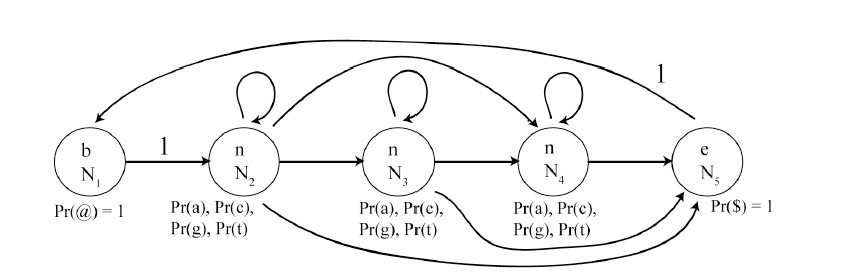
\includegraphics[width=5in]{topolopy_for_training}
  \caption{HMM topology for a DNA sequence of length three.}
  \label{figure:DNAHMM}
\end{figure}



\item	Word classifier: A single model is constructed for the whole vocabulary. 

Generally it’s natural to implement Hidden Markov Models for each of the word when vocabulary is limited and small. And similar topologies can be found among those HMMs. Then we can also use forward and backward algorithm to choose the most likely model to tell which word it is as what we did for character classifier above. It works really well when we classify the test data to get the results within 20 words as following.

["dog","cat","pig","love","hate","scala","python","summer","winter",\\"night",daydream","nightmare","animal","happiness","sadness","tennis",\\"feminism","fascism","socialism","capitalism"]

However, it is time consuming and not realistic to generate HMMs for every word when the vocabulary is relatively large. Therefore, later on we came up with another HMM topology to ideally describe unconstrained words of mixed style.

To be specific, a Hmm  with a topology that is a complete directed graph is modeled. It has 28 hidden states(26 for 26 letters and 2 for @ and \$). See Fiture \ref{figure:wordtopology}. 

\begin{figure}[h!]
  \centering
  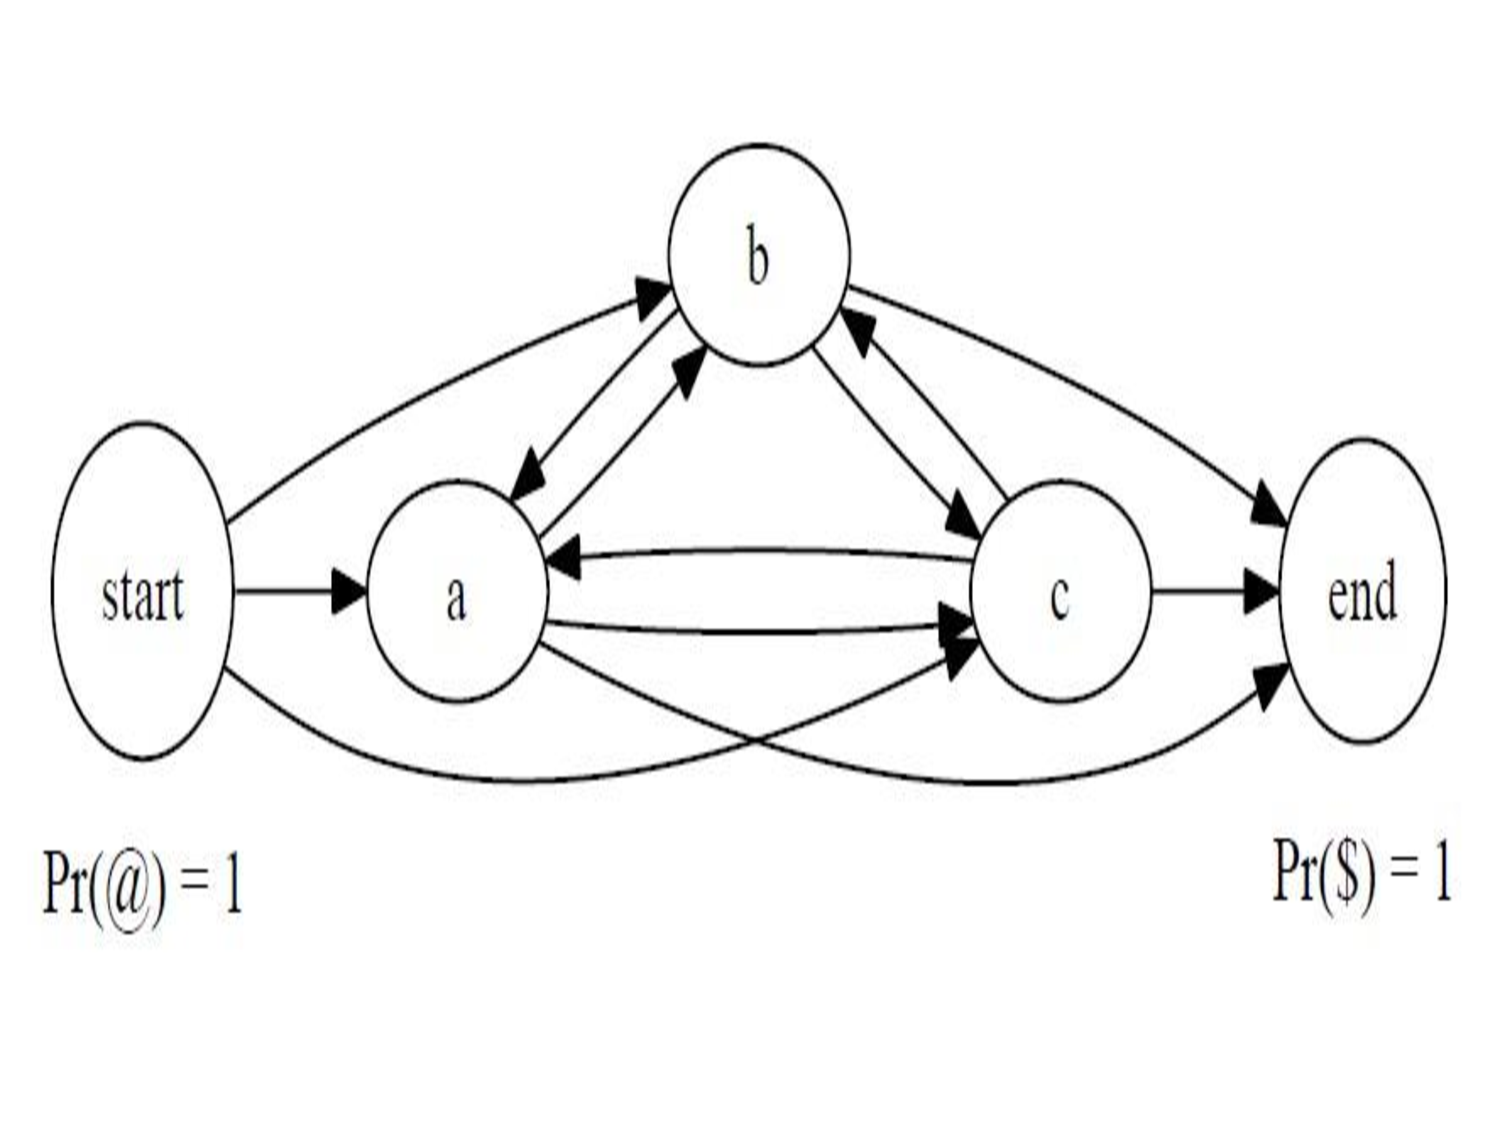
\includegraphics[width=5in]{wordtopology}
  \caption{Word HMM topology for a three-letter alphabet.}
  \label{figure:wordtopology}
\end{figure}


Transition matrix is a 28 * 28 matrix, which is estimated from the lexicon analysis. For example if there's only three words in our vocabulary: dog cat cap for "A to T is set to 0.5 and A to P is set to 0.5" and "A to other letters is set to 0".

Each state's observation is the letter we observed from the character classifier in the previous step. For setting the observation probability matrix, it's reasonable to set them to the probabilities from the test results from word classifier. For example, if we have 10 test examples , for A and 5 of them are classified to be A, 3 to B and 2 to C by the character classifier, then P(observation A)=0.5, P(observation B)=0.3 and P(observation C)=0.2. Then we will assign the row for A as"0.5 0.3 0.2 0 0 ......0 0".

\end{enumerate}

\subsection{prevention of underflow}

For sufficiently large t states, forward variable $\textbf{a}_t(i)$ and backward variable  $\textbf{b}_t(i)$ head exponentially to zero and exceed the precision range of computer. The only reasonable way of performing the computation is by incorporating a scaling procedure[rabineer].
For each t, first we compute $\textbf{a}_t(i)$ according to the induction fomula(20) in rabiner's paper \cite{Rabiner1989},and then multiply it by a scaling factor  $\textbf{c}_t$, where c is equal to $ \frac{1}{ \displaystyle\sum_{i=1}^N \textbf{a}_t(i)}$.

To escape the underflow situation in viterbi algorithm, in order to give the maximum likelihood state sequence, we can simply adopt adding log probability rather than multiplying probabilities. Then no scaling is required.

\subsection{Handling null transitions}
Another problem may occur when training HMM parameters is that transition probability is very likely to be null. In our implementation, we initialze them to very small number, such as \textbf{ $10^{-10}$}.



